%% abtex2-modelo-projeto-pesquisa.tex, v-1.9.7 laurocesar
%% Copyright 2012-2018 by abnTeX2 group at http://www.abntex.net.br/ 
%%
%% This work may be distributed and/or modified under the
%% conditions of the LaTeX Project Public License, either version 1.3
%% of this license or (at your option) any later version.
%% The latest version of this license is in
%%   http://www.latex-project.org/lppl.txt
%% and version 1.3 or later is part of all distributions of LaTeX
%% version 2005/12/01 or later.

\documentclass[
	% -- opções da classe memoir -https://www.folha.uol.com.br/-
	12pt,				% tamanho da fonte
	% openright,			% capítulos começam em pág ímpar (insere página vazia caso preciso)
	oneside,			% para impressão apenas em frente, nao frente verso. Oposto a twoside
	a4paper,			% tamanho do papel. 
	sumario=tradicional,
	% -- opções da classe abntex2 --
% 	chapter=TITLE,		% títulos de capítulos convertidos em letras maiúsculas
	%section=TITLE,		% títulos de seções convertidos em letras maiúsculas
	%subsection=TITLE,	% títulos de subseções convertidos em letras maiúsculas
	%subsubsection=TITLE,% títulos de subsubseções convertidos em letras maiúsculas
	% -- opções do pacote babel --
	english,			% idioma adicional para hifenização
	french,				% idioma adicional para hifenização
	spanish,			% idioma adicional para hifenização
	brazil,				% o último idioma é o principal do documento
]{abntex2}

% ---
% PACOTES
% ---

% ---
% Pacotes fundamentais 
% ---
% \usepackage{helvet}
% \renewcommand{\familydefault}{\sfdefault}
% \usepackage{times}
\usepackage{lmodern}			    % Usa a fonte Latin Modern
\usepackage[T1]{fontenc}		% Selecao de codigos de fonte.
\usepackage[utf8]{inputenc}		% Codificacao do documento (conversão automática dos acentos)
\usepackage{indentfirst}		% Indenta o primeiro parágrafo de cada seção.
\usepackage{color}				% Controle das cores
\usepackage{graphicx}			% Inclusão de gráficos
\usepackage{microtype} 			% para melhorias de justificação
\usepackage{lipsum}				% para geração de dummy text
% ---
\usepackage{todonotes}

\usepackage{float}
\usepackage{amssymb}
\usepackage{amsmath}

\usepackage{mathtools}
% ---
% Pacotes de citações
% ---
% \usepackage[brazilian,hyperpageref]{backref}	 % Paginas com as citações na bibl
\usepackage[alf]{abntex2cite}	% Citações padrão ABNT
\usepackage{subcaption}

\usepackage{listings}

\usepackage{xcolor}

%New colors defined below
\definecolor{codegreen}{rgb}{0,0.6,0}
\definecolor{codegray}{rgb}{0.5,0.5,0.5}
\definecolor{codepurple}{rgb}{0.58,0,0.82}
\definecolor{backcolour}{rgb}{0.95,0.95,0.92}

%Code listing style named "mystyle"
\lstdefinestyle{mystyle}{
	backgroundcolor=\color{backcolour}, commentstyle=\color{codegreen},
	keywordstyle=\color{magenta},
	numberstyle=\tiny\color{codegray},
	stringstyle=\color{codepurple},
	basicstyle=\ttfamily\footnotesize,
	breakatwhitespace=false,         
	breaklines=true,                 
	captionpos=b,                    
	keepspaces=true,                 
	numbers=left,                    
	numbersep=5pt,                  
	showspaces=false,                
	showstringspaces=false,
	showtabs=false,                  
	tabsize=2
}

%"mystyle" code listing set
\lstset{style=mystyle}

\DeclareMathOperator*{\argmin}{argmin}
\DeclarePairedDelimiter\ceil{\lceil}{\rceil}
\DeclarePairedDelimiter\floor{\lfloor}{\rfloor}

% --- 
% % CONFIGURAÇÕES DE PACOTES
% % --- 

% ---
% Informações de dados para CAPA e FOLHA DE ROSTO
% ---
\titulo{Reconstrução de curvas por meio de características robustas extraídas de imagens}
\autor{%
  UNIVERSIDADE DE SÃO PAULO\\Instituto de Ciências Matemáticas e de Computação}
\local{Brasil}
\data{2021}
\instituicao{%
  \textbf{Bolsista:} André Luís Mendes Fakhoury
  \par
  \textbf{Orientador:} João do Espirito Santo Batista Neto}
\tipotrabalho{Iniciação Científica}
\preambulo{Relatório científico final de iniciação científica referente ao processo FAPESP nº 2020/07224-5 para o período entre 01/03/2021 e 30/09/2021.}
% ---

% ---
% Configurações de aparência do PDF final

% alterando o aspecto da cor azul
\definecolor{blue}{RGB}{41,5,195}
\definecolor{black}{RGB}{0,0,0}

% informações do PDF
\makeatletter
\hypersetup{
     	%pagebackref=true,
		pdftitle={\@title}, 
		pdfauthor={André Luís Mendes Fakhoury},
    	pdfsubject={\imprimirpreambulo},
	    pdfcreator={LaTeX with abnTeX2},
		pdfkeywords={abnt}{latex}{abntex}{abntex2}{projeto de pesquisa}, 
		colorlinks=true,       		% false: boxed links; true: colored links
    	linkcolor=black,          	% color of internal links
    	citecolor=black,        		% color of links to bibliography
    	filecolor=magenta,      		% color of file links
		urlcolor=black,
		bookmarksdepth=4
}
\makeatother
% --- 

% --- 
% Espaçamentos entre linhas e parágrafos 
% --- 

% O tamanho do parágrafo é dado por:
\setlength{\parindent}{1.3cm}

% Controle do espaçamento entre um parágrafo e outro:
\setlength{\parskip}{0.2cm}  % tente também \onelineskip
\setlength{\marginparwidth}{2cm}

% \DoubleSpacing

% ---
% compila o indice
% ---
\makeindex
% ---

% ----
% Início do documento
% ----

\begin{document}

% Seleciona o idioma do documento (conforme pacotes do babel)
%\selectlanguage{english}
\selectlanguage{brazil}

% Retira espaço extra obsoleto entre as frases.
\frenchspacing 

% ----------------------------------------------------------
% ELEMENTOS PRÉ-TEXTUAIS
% ----------------------------------------------------------
% \pretextual

% ---
% Folha de rosto
% ---
 \imprimirfolhaderosto
% ---

% ---
% inserir o sumario
% ---
\pdfbookmark[0]{\contentsname}{toc}
\tableofcontents*
\cleardoublepage
% ---

% ----------------------------------------------------------
% ELEMENTOS TEXTUAIS
% ----------------------------------------------------------
\textual
\pagestyle{simple}

\begingroup
\let\clearpage\relax

% ----------------------------------------------------------
% Organização
% ----------------------------------------------------------

\chapter{Introdução}\label{ch::intro}
Este documento tem como objetivo apresentar as atividades realizadas pelo bolsista André Luís Mendes Fakhoury no período de outubro de 2020 a março de 2021, referente ao projeto de Iniciação Científica, processo FAPESP nº 2020/07224-5. O trabalho, intitulado ``Reconstrução de curvas por meio de características robustas extraídas de imagens'', é parte de umas das linhas de pesquisa do projeto temático FAPESP de nº 2019/07316-0, que visa a reconstrução de faces humanas a partir de informações reduzidas do domínio.


\section{O projeto e cronograma original}

Um dos desafios encontrados em visão computacional é o mapeamento de características robustas entre espaços bidimensionais e tridimensionais. Este processo pode ser simplificado com a redução de informações a serem analisadas: como representar curvas a partir de algum conjunto reduzido de pontos.

Este projeto visa, principalmente, a extração de características robustas de curvas, e posterior reconstrução delas a partir destas informações reduzidas com um erro mínimo. Os pontos que representam estas características robustas são denominados pontos importantes.

Para este processo, contornos de imagens podem ser extraídos e analisados como curvas discretas e, portanto, reduzidos a finitos pontos importantes. A partir desta premissa, os seguintes objetivos específicos podem ser definidos:

\begin{itemize}[noitemsep]
	\item Extrair características robustas em $\mathbb{R}^2$ para reconstrução de curvas com alta precisão a partir de imagens. 
	\item Pré-processar as imagens com eliminação de ruídos, binarização e consequente segmentação;
	\item Extrair atributos de formas das imagens (contorno e cálculo da curvatura);
	\item Determinar as características robustas por análise da curvatura;
	\item Reconstruir as formas a partir das características robustas, por meio de curvas poligonais e operadores Laplacianos como sugerido por \citeonline{Sorkine2006} e 
	\item Aferir a qualidade da reconstrução a partir da curva original.
\end{itemize}

As principais etapas de desenvolvimento deste projeto são ilustradas no diagrama de blocos da figura \ref{fig:diagrama}. O projeto, como inicialmente proposto, apresentou o cronograma representado na tabela \ref{tab:cronograma}.

\begin{figure}[htb]
	\centering
	\caption{Diagrama de bloco das etapas de desenvolvimento}
	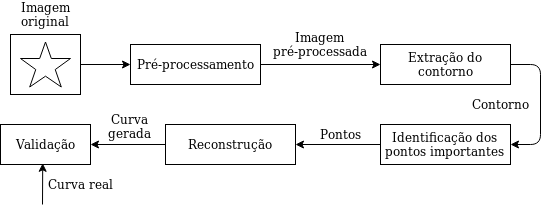
\includegraphics[width=.7\linewidth]{./img/diagrama.png}
	\legend{Fonte: Elaborada pelo autor.}
	\label{fig:diagrama}
\end{figure}



\begin{table}[htb]
	\footnotesize
	\centering
	\vspace{0.5em}
	\setlength{\tabcolsep}{0.05in}
	\begin{tabular}{|c|c|c|c|c|c|c|}
		\hline
		Atividades
		& \multicolumn{6}{c|}{Meses de trabalho} \\
		\cline{2-7}
		& 1\textordmasculine\ e 2\textordmasculine & 3\textordmasculine\  e 4\textordmasculine & 5\textordmasculine\  e 6\textordmasculine & 7\textordmasculine\  e 8\textordmasculine & 9\textordmasculine\  e 10\textordmasculine & 11\textordmasculine\  e 12\textordmasculine \\ \hline
		Estudo das técnicas de reconstrução de curvas  & $\bullet$ & $\bullet$ & & & &\\ \hline
		Pré-processamento e Extração de contornos & & $\bullet$ & $\bullet$ & & & \\ \hline
		Extração dos pontos importantes & & $\bullet$ & $\bullet$ & & & \\ \hline
		Redação do relatório parcial & & & $\bullet$ & & & \\ \hline
		Implementação da reconstrução de curvas & & & & & & \\
		(Sorkine)& & & $\bullet$ & $\bullet$ & $\bullet$ & \\ \hline
		Avaliação e testes & & & & $\bullet$ & $\bullet$ & \\ \hline
		Desenvolvimento do relatório final & & & & & $\bullet$ & $\bullet$ \\ \hline
	\end{tabular}
	\caption{Cronograma de atividades para 12 meses de trabalho.}
	\label{tab:cronograma}
\end{table}

\section{Reordenação do cronograma}\label{sec::reordenacao}

Durante o segundo semestre de 2020, o professor Dr. Antônio Castelo Filho, pesquisador principal do projeto temático, lecionou a disciplina ``Modelagem Geométrica'', de código SME0271, para alunos de graduação e com espelho em ``Tópicos em Análise Numérica II (Variedades Computacionais)'', de código SME5850, para a pós-graduação. Nela, foram abordados diversos tópicos referentes a variedades computacionais. Nas reuniões semanais de acompanhamento das atividades do temático por cada membro da equipe,  o prof. Castelo e demais pesquisadores incentivaram ao aluno bolsista e demais colegas a cursar a disciplina, visto ser uma grande oportunidade para adquirir conhecimento sobre a modelagem geométrica e análise numérica das várias linhas de pesquisas relacionadas. No caso particular deste projeto, a atividade diretamente relacionada referiu-se à reconstrução de curvas pelo método descrito em \citeonline{Sorkine2006}, originalmente programada para ser desenvolvida na segunda metade deste projeto. 

Além do aluno bolsista deste projeto, três alunos de mestrado do projeto temático cursaram a disciplina. Uma das formas de avaliação da disciplina era a co-autoria da escrita de um capítulo de um livro, que ainda será publicado.

Como resultado, a atividade 5 (implementação da reconstrução de curvas) foi antecipada e a atividade 3 (extração dos pontos importantes) postergada para os próximos meses, sem prejudicar o desenvolvimento do projeto. Ressalto que cursar a disciplina foi muito compensador, tendo contribuído para um melhor entendimento da teoria de reconstrução de curvas a partir de um conjunto de pontos e, sobretudo, no momento da implementação, a ser apresentada neste relatório.

\section{Organização do relatório}

As próximas seções deste relatório serão estruturadas da seguinte maneira:

\begin{itemize}[noitemsep]
	\item Na seção \ref{ch::realizadas} serão descritos alguns conceitos estudados e as atividades realizadas;
	\item Na seção \ref{ch::proximas} serão vistas as próximas atividades a serem realizadas;
% 	\item Na seção \ref{ch::consideracoes} serão dadas algumas considerações finais.
\end{itemize}

\chapter{Atividades realizadas}\label{ch::realizadas}
Nesta seção serão relatadas as atividades desenvolvidas pelo aluno bolsista nesta segunda metade do projeto. A seção \ref{sec:extracao} descreve o processo de extração dos pontos importantes da curva discreta obtida da imagem. A seção \ref{sec:combinacao} contém o que foi desenvolvido na etapa de combinação dos algoritmos, com a respectiva fonte para os códigos desenvolvidos. Por último, a etapa \ref{sec:avaliacao} ilustra os resultados obtidos, nos diferentes tipos de imagens e malhas utilizados para os testes.

\section{Extração dos pontos importantes}\label{sec:extracao}

A extração de pontos importantes consistem em, a partir de um conjunto finito de $n$ pontos, que representa uma curva discreta, computar os índices dos pontos âncora que serão utilizados pelo algoritmo de reconstrução. A quantidade de pontos a serem escolhidos também é enviada por parâmetro.

Alguns métodos foram considerados para a seleção dos pontos importantes. Foram eles:

\begin{itemize}
    \item \textbf{Pontos linearmente espaçados:} os pontos são escolhidos de modo que os índices sejam igualmente espaçados entre si.
    \item \textbf{Escolha aleatória de pontos:} os pontos são escolhidos de modo aleatório, apenas tomando cuidado para que não sejam muito próximos um do outro.
    \item \textbf{Escolha de pontos pela curvatura:} inicialmente é calculada a curvatura discreta da curva em cada ponto, e aqueles com maior valor absoluto são escolhidos.
\end{itemize}

Destes, serão analisados resultados encontrados utilizando pontos linearmente espaçados e pela curvatura. A escolha de pontos igualmente espaçados pode ser realizada facilmente utilizando a função \texttt{linspace} em linguagens como Python e MATLAB. Já para a escolha de pontos pela curvatura é previamente necessária a análise da curva discreta. Para isso, será revisada a teoria da análise de curvatura discreta.

A curvatura de uma curva regular parametrizada por uma aplicação $t \rightarrow (x(t), y(t))$, onde $x(t)$ e $y(t)$ são funções de classe $C^2$, é dada por \cite{OliveiraMarroquim2020}:

\begin{equation}
	\kappa (t) = \frac{x'(t) y''(t) - y'(t) x''(t)}{(x'(t)^2 + y'(t)^2)^{3/2}}.
\end{equation}

No projeto, as curvas não são contínuas, mas sim representadas por um conjunto discreto de pontos $(x, y)$ - que representam a posição de cada pixel. Por isso, as derivadas mostradas na equação acima devem ser calculadas de maneira discreta. Uma das maneiras de se calcular isto é partir de métodos espectrais de Fourier \cite{brethwashington}.

Seja $u_j$ uma aproximação discreta da função $u(x)$, com $n$ pontos de amostra $x_j \in h, 2h, \dots, ih, \dots, 2\pi - h, 2\pi$, onde $h = 2\pi/n$. Para o caso discreto, pode-se aplicar a versão computacionalmente otimizada da transformada de Fourier (FFT) em $u_j$, tal que $FFT(u_j) \equiv \hat{u}_k$, em que $k \in \frac{-n}{2}+1, \dots, \frac{n}{2}$. Sabe-se que:

$$FFT \left (\frac{\partial u_j}{\partial x} \right) \equiv i k \hat{u}_k$$

Assim, para obter o valor da derivada, basta calcular a transformada rápida inversa IFFT. O código calcula a derivada de uma função discreta $y$ no domínio $x$ e emprega um filtro Gaussiano com fator de suavização $\sigma$. A aplicação de um filtro Gaussiano no cálculo da derivada tem por objetivo evitar a amplificação do efeito de serrilhamento (\textit{aliasing}), quando houver, causado pela transformada de Fourier \cite{li1987}. O filtro Gaussiano cumpre este objetivo ao eliminar altas frequências presentes no sinal com a propriedade de preservar a localização de pontos importantes da mudança da curvatura \cite{tomasi2007}.

Com a curvatura de cada ponto calculada, é necessário escolher os pontos que serão utilizados como âncoras para representar a curva. Porém, uma  escolha simples dos pontos com maior curvatura pode fazer com que algumas regiões do contorno sejam super-representadas, enquanto outras fiquem sem pontos âncora.

Por isso, a estratégia utilizada foi a seguinte: 25\% dos pontos serão escolhidos de forma linear. Os outros 75\% serão enfim escolhidos por possuírem maior valor absoluto de curvatura. Para que os pontos sejam mais bem distribuídos por todo o contorno, antes de um ponto ser adicionado é feita uma verificação se este possui algum vizinho muito próximo presente no conjunto de pontos âncora já escolhidos. Caso o ponto não tenha vizinhos já adicionados no conjunto de pontos escolhidos, este pode ser então adicionado. A quantidade de vizinhos a serem analizados é constantemtente subtraída para que não haja laços de repetição infinitos. O trecho de código fonte abaixo descreve este processo.

\begin{lstlisting}[language=Python]
# calculo da curvatura e ordenacao dos pontos por isso
kappa = calc_curvature(contour[:,0], contour[:,1], np.arange(n))
arr = sorted([(np.abs(kappa[i]), i) for i in range(n)], reverse=True)

# escolha de 25% dos pontos de forma linear
chosen = set(np.linspace(0, n - 1, qtt//4).astype(int))

# inicia com um range maior e depois diminui
delta_range = n // 20
while len(chosen) < qtt:
  for curv, idx in arr:
    can_be = len(chosen) < qtt

  # verifica se vizinhos proximos ja estao adicionados
  for delta in range(-delta_range, delta_range):
    can_be = can_be and not (idx + delta) % n in chosen

  # pode ser adicionado no conjunto
  if can_be:
    chosen.add(idx)

  # diminui o intervalo de verificacao (evitar loops infinitos)
  delta_range = max(delta_range - 5, 0)
\end{lstlisting}

\section{Combinação dos algoritmos}\label{sec:combinacao}

Nesta seção do projeto foi implementado um \textit{notebook} em Python que organiza todas as etapas de desenvolvimento do projeto. A versão final \cite{Fakhoury2021} foi disponibilizada no GitHub\footnote{Disponível em <https://github.com/andrefakhoury/image-curve-reconstruction>. Acesso em 8 out 2021.}.

Em grande parte, os procedimentos que envolvem imagens foram tratados com a biblioteca \citeonline{OpenCV}. As operações matriciais foram resolvidas utilizando NumPy e os gráficos feitos com a biblioteca MatPlotLib.

O \textit{notebook} está organizado nas seguintes seções:

\begin{itemize}[noitemsep]
\item \textbf{Pré-processamento} - incluindo a extração dos contornos;
\item \textbf{Processamento de curvas} - a partir do conjunto de coordenadas $(x, y)$ de cada ponto, pode ser calculada a curvatura discreta;
\item \textbf{Escolha dos pontos âncora} - possibilidade de escolha dos pontos como descrito na seção anterior (\ref{sec:extracao});
\item \textbf{Reconstrução} - funções de reconstrução descritas em \citeonline{Sorkine2006};
\item \textbf{Testes} - finalmente, avaliações e testes, como serão descritas na seção \ref{sec:avaliacao}.
\end{itemize}

\section{Avaliação e testes}\label{sec:avaliacao}

Na etapa final do projeto foram realizados testes com diversas imagens, curvas e malhas. Primeiramente serão descritas as análises utilizando as imagens de folhas do repositório \citeonline{imageclef2011} - inicialmente descrito no projeto como o banco de dados a ser testado - e, posteriormente, testes em curvas abertas e fechadas em $\mathbb{R}^2$ e $\mathbb{R}^3$. Também foram realizados testes em malhas poligonais, que serão descritos no último tópico desta seção.

O erro será computado como sendo a distância euclidiana entre cada ponto da curva original e da curva reconstruída: para cada índice de vértice $i$, o erro dos pontos obtidos $\mathbf{v'}$ em relação aos pontos originais $\mathbf{v}$ é:

$$E_i(\mathbf{v, v'}) = \sqrt{(\mathbf v_i^{(x)} - \mathbf v_i'^{(x)})^2 + (\mathbf v_i^{(y)} - \mathbf v_i'^{(y)})^2}$$

\noindent e o erro total da reconstrução é calculado como a soma dos erros para cada ponto:

$$E(\mathbf{v, v'}) = \sum_{i = 1}^{|V|}E_i(\mathbf{v, v'})$$

\subsection{Imagens de folhas do repositório \citeonline{imageclef2011}}

Os primeiros exemplos analisados foram imagens de folhas de árvores, retiradas do repositório do \citeonline{imageclef2011}. Este banco de imagens foi citado no projeto original, e utilizado com a justificativa de que os contornos das figuras podem ser extraídos com alta precisão, facilitando a avaliação do método.


\begin{figure}[H]
	\centering
	\begin{subfigure}[b]{\textwidth}
		\centering
		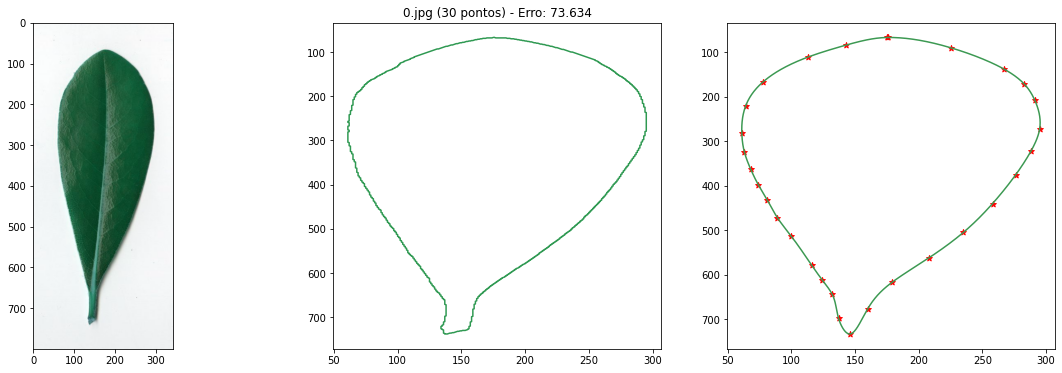
\includegraphics[width=0.9\textwidth]{img/res/0_30.png}
		\caption{Erro = 73.63.}
	\end{subfigure}
	\\
	\begin{subfigure}[b]{\textwidth}
		\centering
		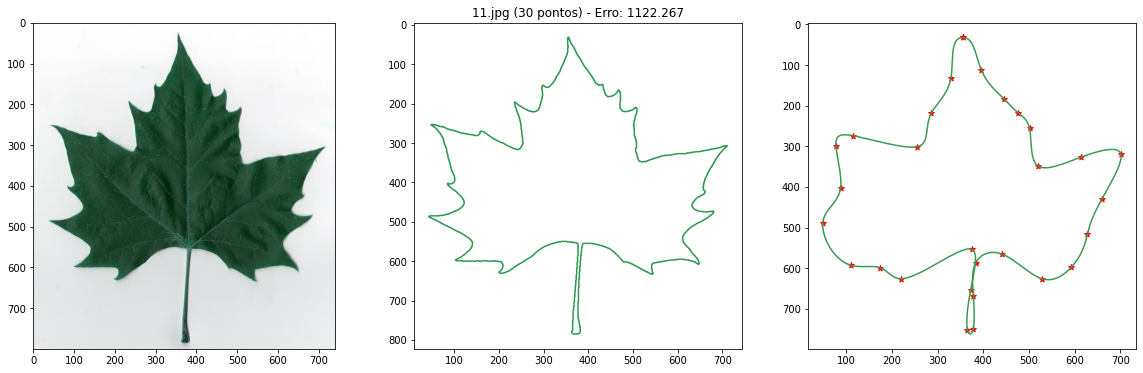
\includegraphics[width=0.9\textwidth]{img/res/1_30.png}
		\caption{Erro = 1122.27.}
	\end{subfigure}
	\\
	\begin{subfigure}[b]{\textwidth}
		\centering
		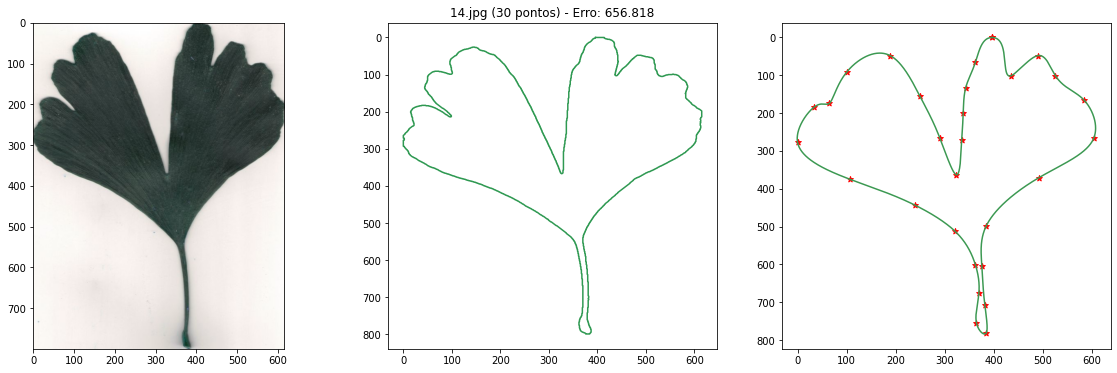
\includegraphics[width=0.9\textwidth]{img/res/2_30.png}
		\caption{Erro = 658.82.}
	\end{subfigure}
	\\
	\begin{subfigure}[b]{\textwidth}
		\centering
		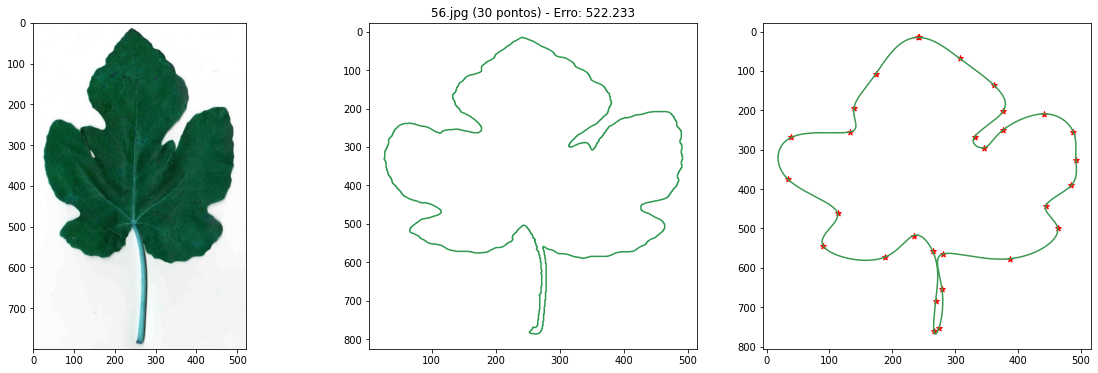
\includegraphics[width=0.9\textwidth]{img/res/3_30.png}
		\caption{Erro = 522.23.}
	\end{subfigure}
	\caption{Representação de folhas utilizando apenas 30 pontos como âncora.}
	\label{fig:folha1rep}
\end{figure}


\begin{figure}[H]
	\centering
	\begin{subfigure}[b]{\textwidth}
		\centering
		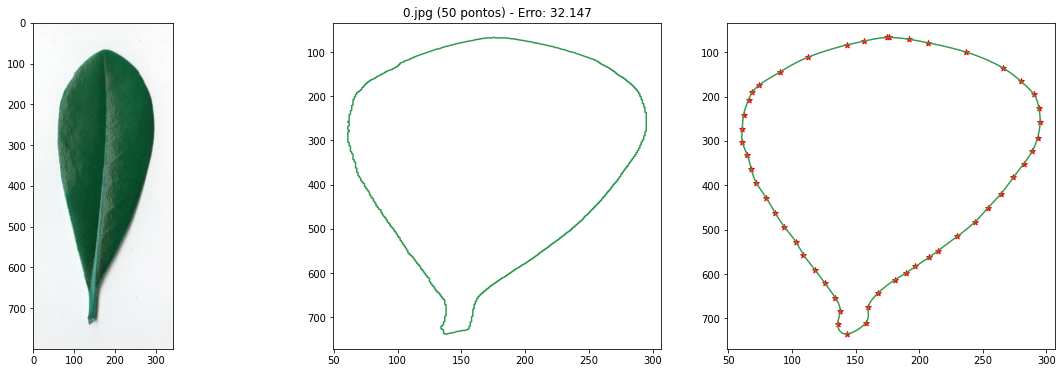
\includegraphics[width=0.9\textwidth]{img/res/0_50.png}
		\caption{Erro = 32.15.}
	\end{subfigure}
	\\
	\begin{subfigure}[b]{\textwidth}
		\centering
		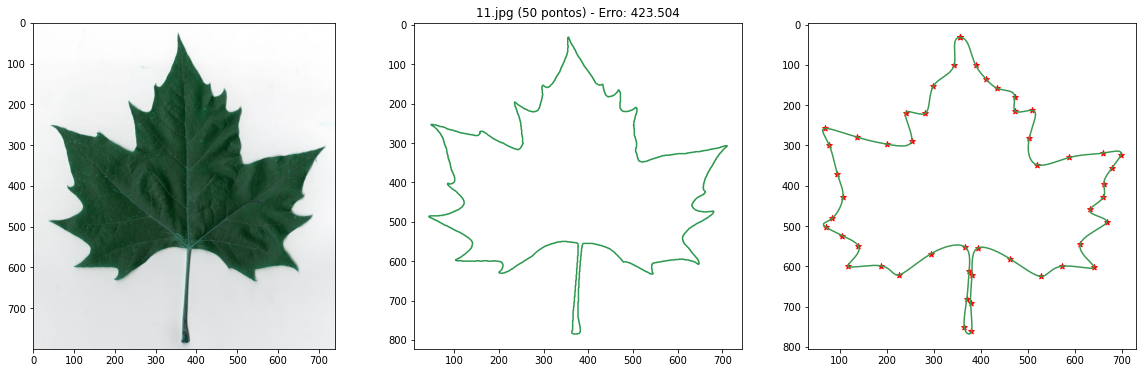
\includegraphics[width=0.9\textwidth]{img/res/1_50.png}
		\caption{Erro = 423.50.}
	\end{subfigure}
	\\
	\begin{subfigure}[b]{\textwidth}
		\centering
		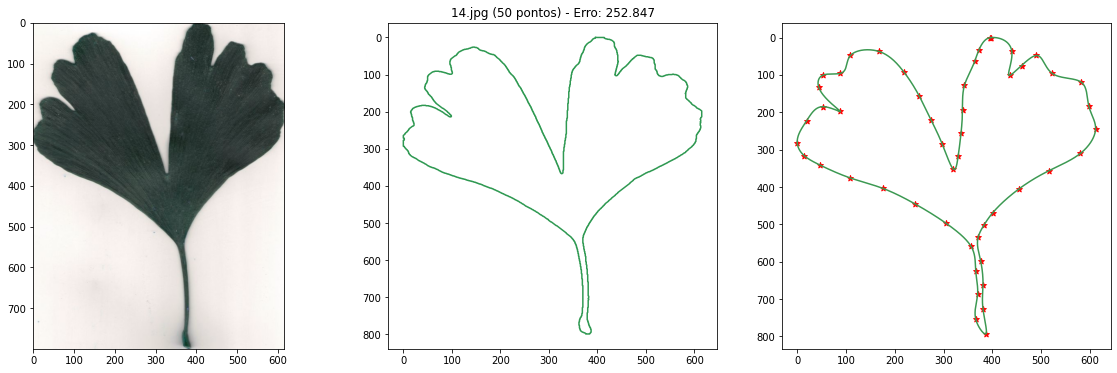
\includegraphics[width=0.9\textwidth]{img/res/2_50.png}
		\caption{Erro = 252.85.}
	\end{subfigure}
	\\
	\begin{subfigure}[b]{\textwidth}
		\centering
		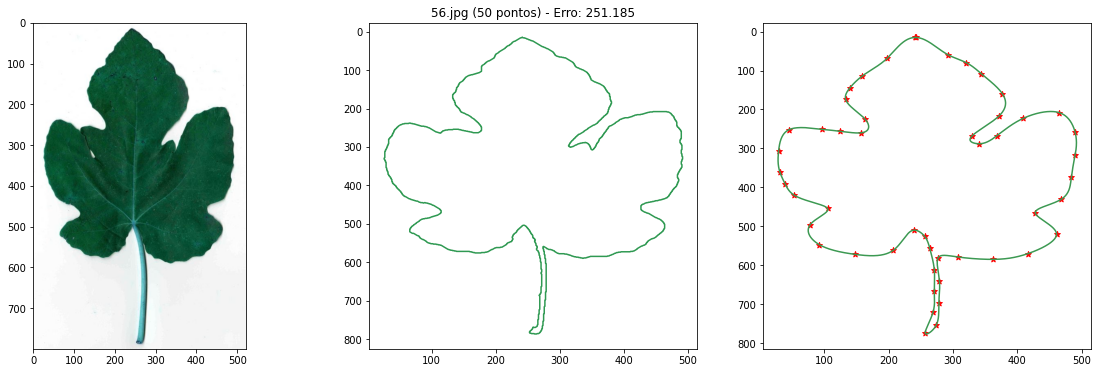
\includegraphics[width=0.9\textwidth]{img/res/3_50.png}
		\caption{Erro = 251.18.}
	\end{subfigure}
	\caption{Representação de folhas utilizando apenas 50 pontos como âncora.}
	\label{fig:folha2rep}
\end{figure}


\begin{figure}[H]
	\centering
	\begin{subfigure}[b]{\textwidth}
		\centering
		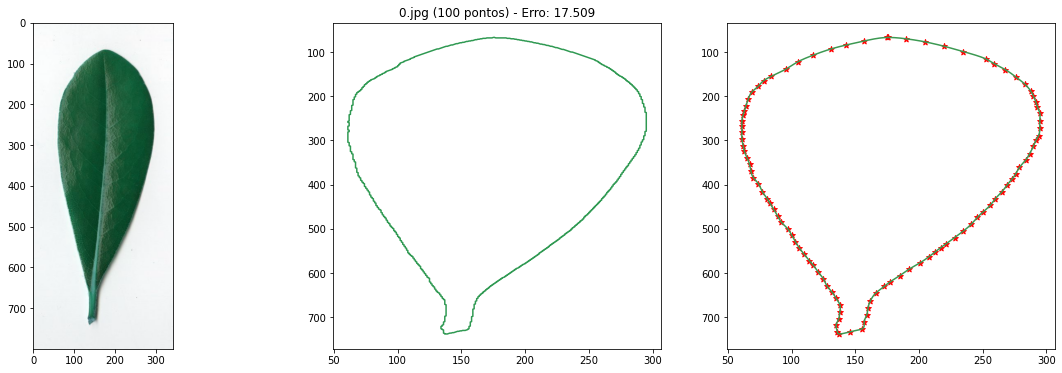
\includegraphics[width=0.9\textwidth]{img/res/0_100.png}
		\caption{Erro = 17.51.}
	\end{subfigure}
	\\
	\begin{subfigure}[b]{\textwidth}
		\centering
		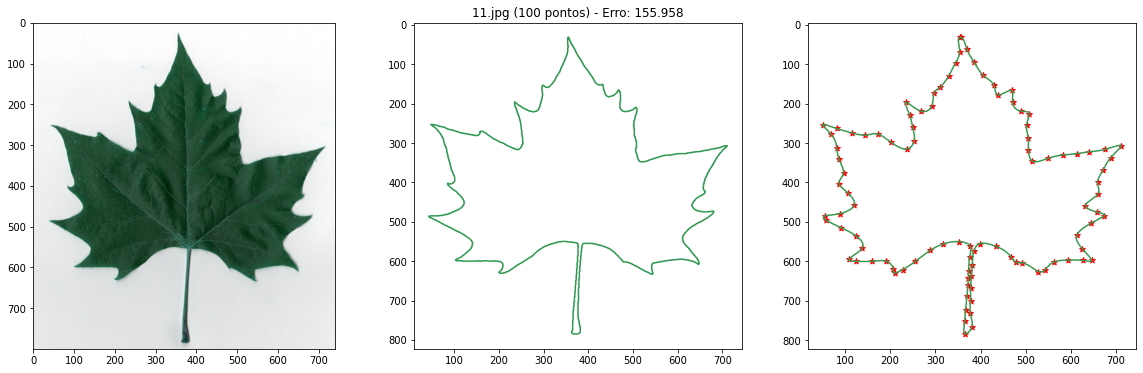
\includegraphics[width=0.9\textwidth]{img/res/1_100.png}
		\caption{Erro = 155.96.}
	\end{subfigure}
	\\
	\begin{subfigure}[b]{\textwidth}
		\centering
		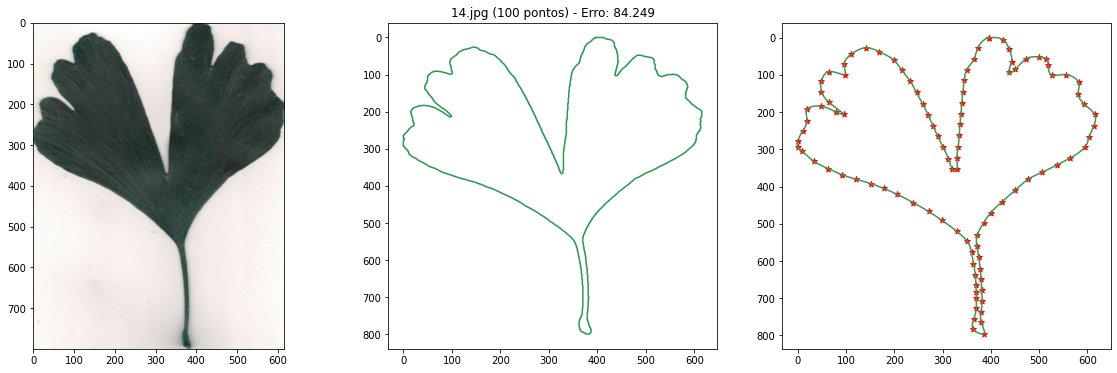
\includegraphics[width=0.9\textwidth]{img/res/2_100.png}
		\caption{Erro = 84.25.}
	\end{subfigure}
	\\
	\begin{subfigure}[b]{\textwidth}
		\centering
		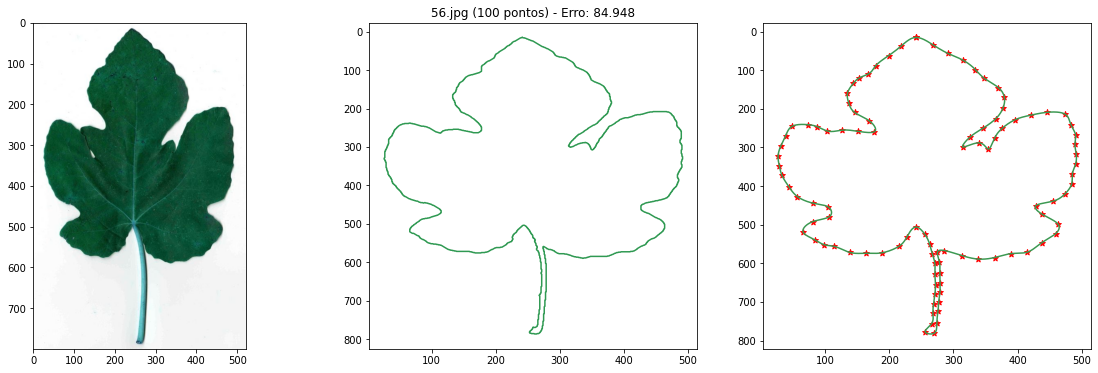
\includegraphics[width=0.9\textwidth]{img/res/3_100.png}
		\caption{Erro = 84.95.}
	\end{subfigure}
	\caption{Representação de folhas utilizando apenas 100 pontos como âncora.}
	\label{fig:folha3rep}
\end{figure}

As figuras \ref{fig:folha1rep}, \ref{fig:folha2rep} e \ref{fig:folha3rep} apresentam os resultados para quatro folhas distintas. Em cada uma delas, há 3 colunas: a primeira mostra a figura original, a segunda o contorno extraído e a terceira mostra a curva reconstruída, com os pontos âncora destacados com estrelas.

\subsection{Curvas abertas e em $\mathbb{R}^3$}

Outros testes foram realizados sobre curvas (discretizadas) abertas e fechadas, em domínios $\mathbb{R}^2$ e $\mathbb{R}^3$. De acordo com \citeonline{Sorkine2006}, o método de reconstrução funciona para quaisquer malhas que sejam aproximações lineares por partes de uma superfície suave.

A figura \ref{fig:c2d1} ilustra um exemplo de reconstrução de uma função paramétrica em $\mathbb{R}^2$ e fechada. A figura \ref{fig:c2d2} mostra um exemplo de função paramétrica em $\mathbb{R}^2$ e aberta. Em ambas, a figura à esquerda mostra a curva original, a do meio os pontos âncora escolhidos e a curva reconstruída a figura à direita.

\begin{figure}[H]
	\centering
	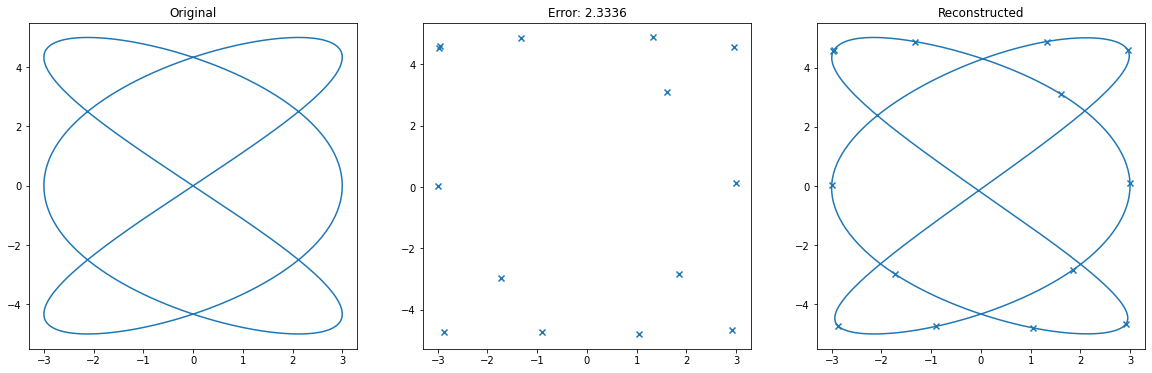
\includegraphics[width=1\textwidth]{img/res/closed2d.png}
	\caption{Representação da função paramétrica $(x(t), y(t)) = (3 cos(3t), 5sen(2t))$, com $t \in [0, 2\pi]$, utilizando 13 pontos como amostra.}
	\label{fig:c2d1}
\end{figure}

\begin{figure}[H]
	\centering
	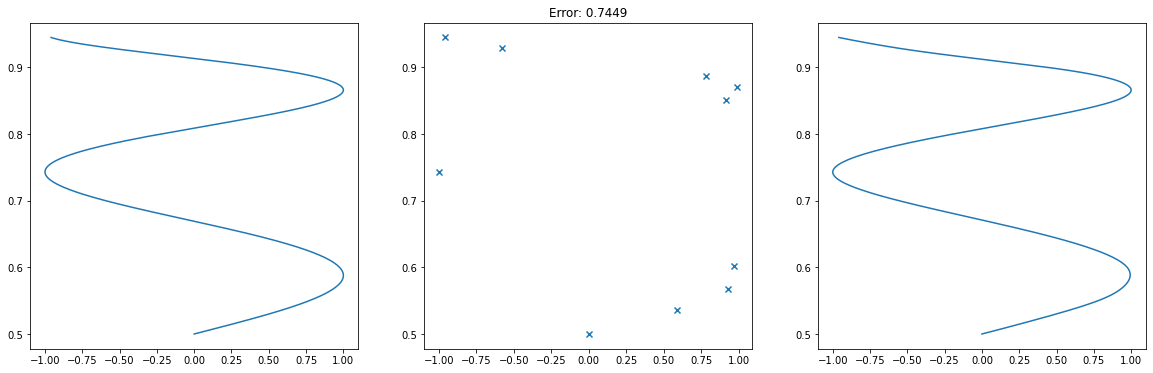
\includegraphics[width=1\textwidth]{img/res/open2d.png}
	\caption{Representação da função paramétrica $(x(t), y(t)) = (sin(5t), cos(t/3))$, com $t \in [1, \pi]$, utilizando 10 pontos como amostra.}
	\label{fig:c2d2}
\end{figure}

A figura \ref{fig:c3d1} mostra um exemplo de representação de uma curva paramétrica aberta em $\mathbb{R}^3$. A imagem à esquerda representa a curva original e a imagem à direita apresenta a curva reconstruída com os pontos âncora destacados. Neste caso, foram escolhidos pontos âncora linearmente espaçados.

\begin{figure}[H]
	\centering
	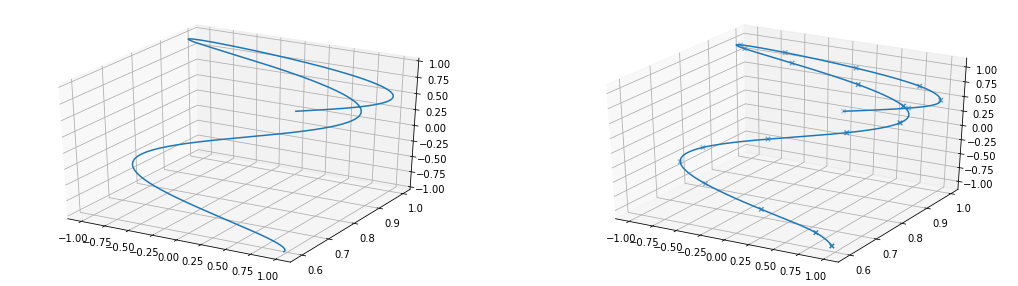
\includegraphics[width=1\textwidth]{img/res/open3d.png}
	\caption{Representação da função paramétrica $(x(t), y(t), z(t)) = (sin(3t), cos(t/5), sin(t))$, com $t \in [0, 1.5\pi]$, utilizando 20 pontos como amostra. Erro = 0.67.}
	\label{fig:c3d1}
\end{figure}

\subsection{Malhas poligonais}

Também foram realizados testes em malhas poligonais tridimensionais. Nestes exemplos, os pontos âncora foram escolhidos a partir de índices linearmente espaçados entre si. Por isso, pode-se destacar visualmente que alguns detalhes foram perdidos.

A figura \ref{fig:ex4rep} mostra exemplo de reconstrução na malha de um coelho utilizando-se apenas uma amostra dos pontos. A quantidade de pontos utilizadas em cada exemplo encontra-se na legenda de cada figura.

\begin{figure}[H]
	\centering
	\begin{subfigure}[b]{0.47\textwidth}
		\centering
		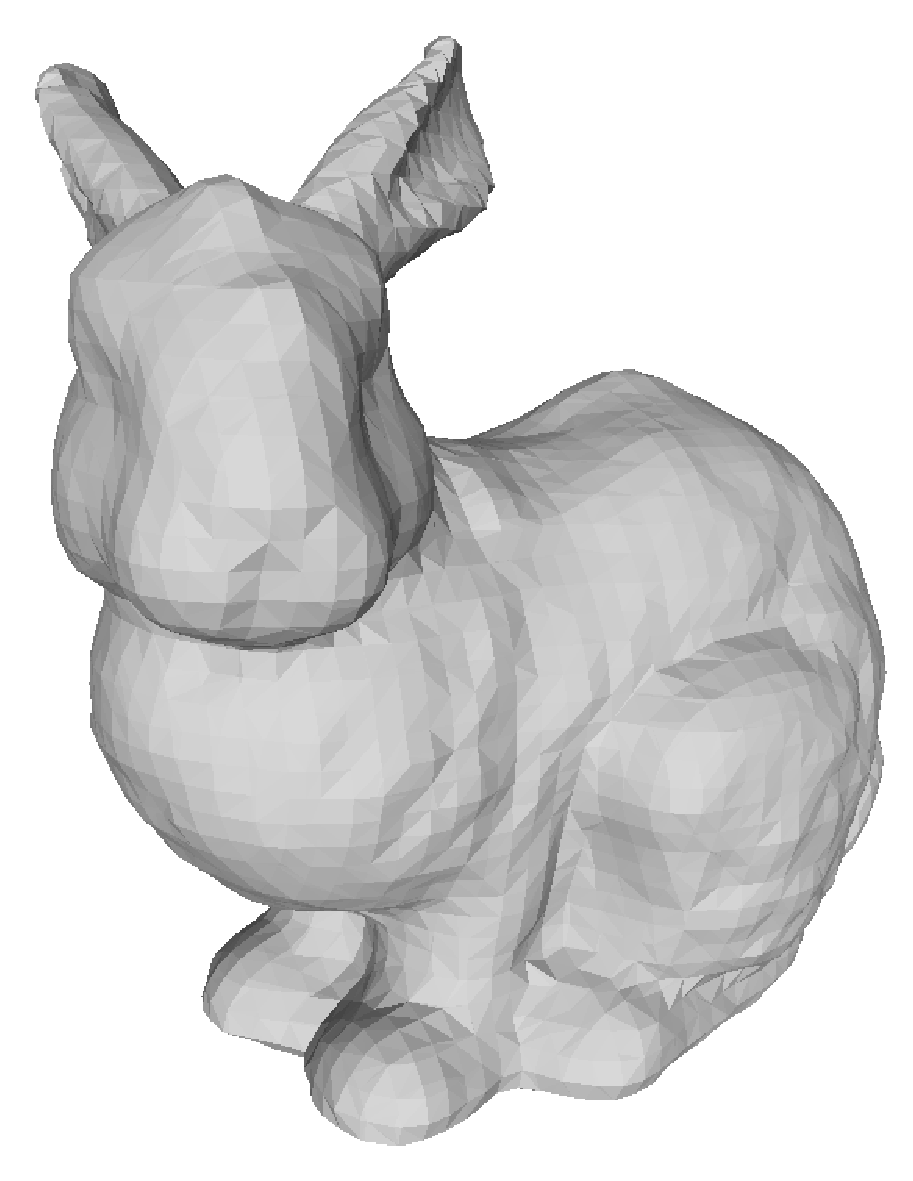
\includegraphics[width=0.43\textwidth]{img/res/bunny_all.eps}
		\caption{Malha original}
		\label{fig:ex41}
	\end{subfigure}
	\hfill
	\begin{subfigure}[b]{0.47\textwidth}
		\centering
		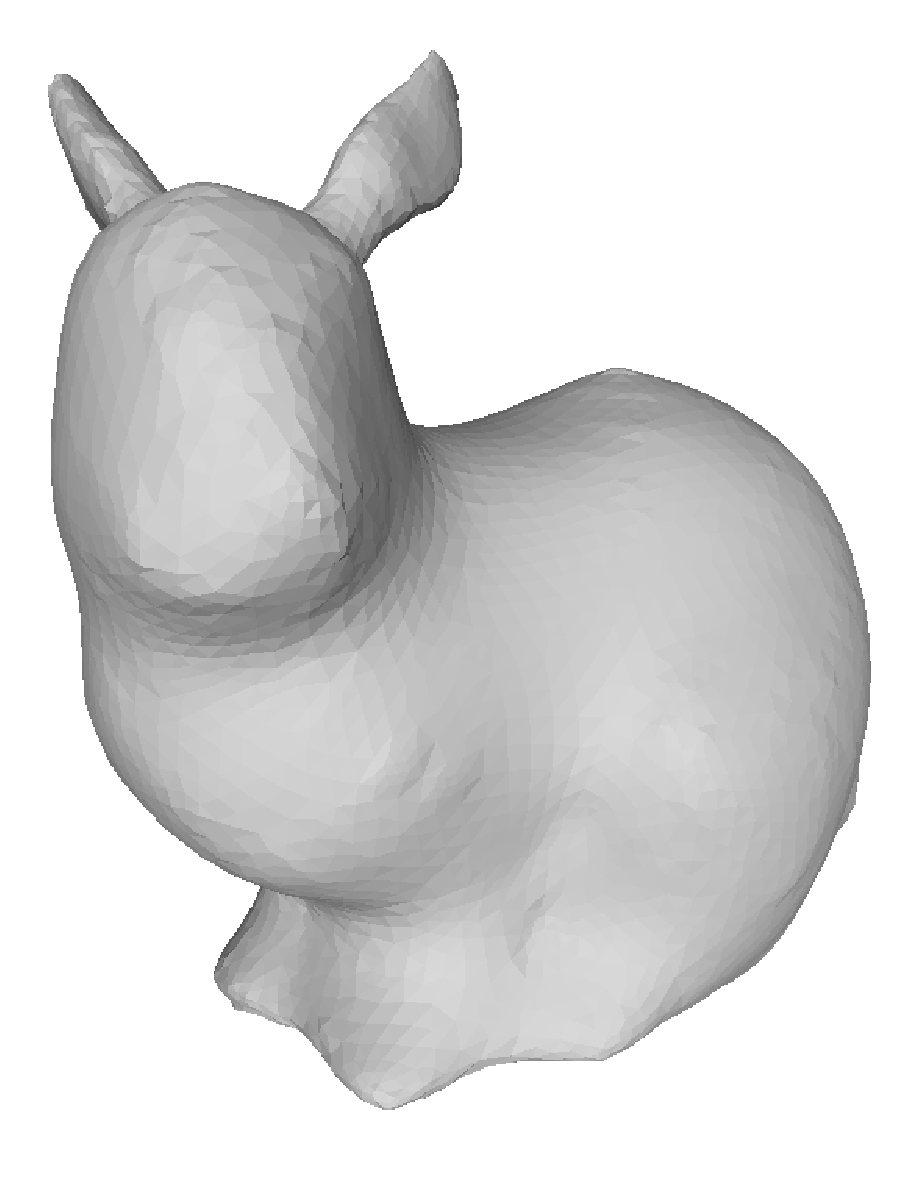
\includegraphics[width=0.43\textwidth]{img/res/bunny_10.eps}
		\caption{10\% dos pontos. Erro = 1037.08.}
		\label{fig:ex42}
	\end{subfigure}
	\\
	\begin{subfigure}[b]{0.47\textwidth}
		\centering
		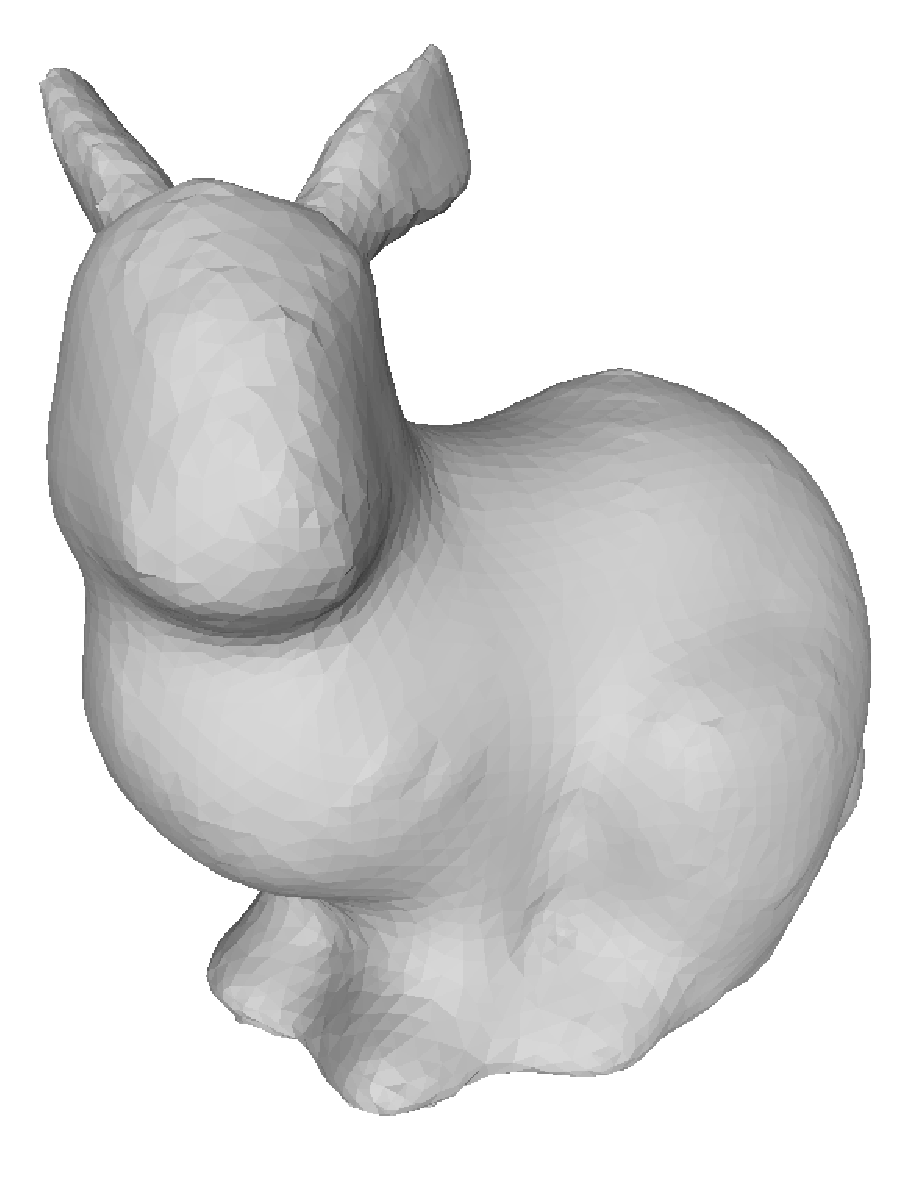
\includegraphics[width=0.43\textwidth]{img/res/bunny_30.eps}
		\caption{30\% dos pontos. Erro = 742.05.}
		\label{fig:ex43}
	\end{subfigure}
	\hfill
	\begin{subfigure}[b]{0.47\textwidth}
		\centering
		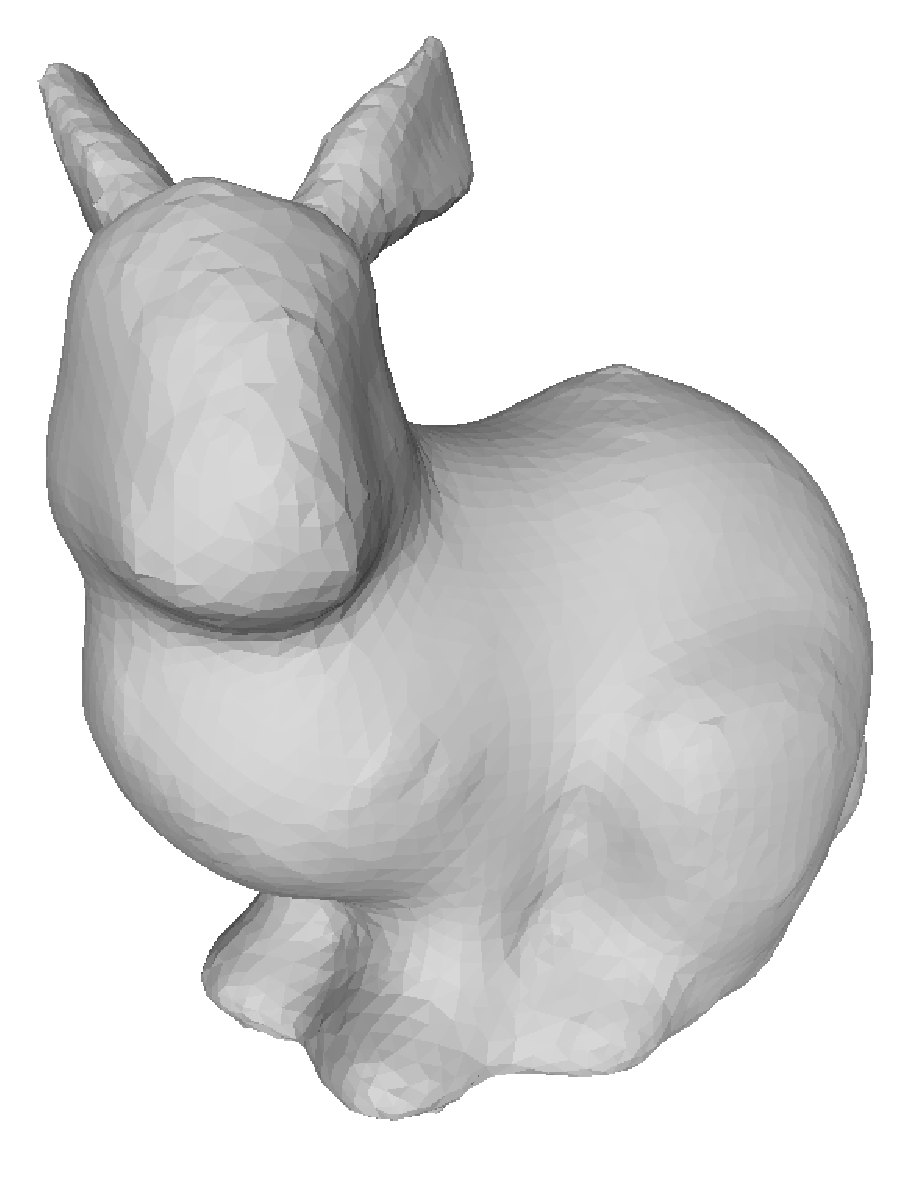
\includegraphics[width=0.43\textwidth]{img/res/bunny_50.eps}
		\caption{50\% dos pontos. Erro = 590.66.}
		\label{fig:ex44}
	\end{subfigure}
	\caption{Representação da malha de um coelho, utilizando apenas uma amostra dos pontos originais como âncoras.}
	\label{fig:ex4rep}
\end{figure}

\chapter{Considerações finais}\label{ch::consideracoes}
Nesta seção serão descritas algumas atividades adicionais realizadas pelo bolsista ao decorrer do projeto.

Durante todo o período referente ao projeto foram realizadas reuniões semanais com o grupo de professores e alunos do projeto temático em que esta iniciação científica está inserida. Nestas, foram preparados e apresentados alguns seminários, que serviram para que todos pudessem acompanhar o andamento do projeto de todos, dar \textit{feedbacks} e planejar os próximos passos a serem executados.

Outro tópico relacionado com o projeto (e que também foi apontado no relatório parcial) foi que, durante o segundo semestre de 2020, o professor Dr. Antônio Castelo Filho, pesquisador principal do projeto temático, lecionou a disciplina ``Modelagem Geométrica'' para alunos de graduação e com espelho em ``Tópicos em Análise Numérica II (Variedades Computacionais)'' para a pós-graduação. Nela, foram abordados diversos tópicos referentes a variedades computacionais. No caso particular deste projeto, a atividade diretamente relacionada referiu-se à representação de curvas em coordenadas diferenciais pelo método descrito em \citeonline{Sorkine2006}. Nesta disciplina, cada estudante participou ativamente no desenvolvimento de um capítulo de um livro, que ainda será publicado.

Além disso, também foram realizados dois \textit{workshops} relacionados ao projeto temático, em que o bolsista participou como ouvinte. O último tópico a ser mencionado é a participação deste projeto no Simpósio Internacional de Iniciação Científica e Tecnológica da USP (SIICUSP) de 2021, que será realizado em outubro de 2021.

Este relatório teve como objetivo listar as atividades realizadas no período de março a setembro de 2021 e exibir um panorama geral de desenvolvimento do projeto. Apesar de algumas dificuldades encontradas na pandemia de COVID-19 e de alterações sobre o cronograma original, pode-se finalizar o projeto no tempo previsto e foi possível promover conhecimento entre os membros do grupo de pesquisa do projeto temático em que este está inserido.


\endgroup
% ----------------------------------------------------------
% ELEMENTOS PÓS-TEXTUAIS
% ----------------------------------------------------------

\postextual

% ----------------------------------------------------------
% Referências bibliográficas
% ----------------------------------------------------------
\bibliography{referencias}

%---------------------------------------------------------------------
% INDICE REMISSIVO
%---------------------------------------------------------------------
\phantompart

\printindex

\end{document}